% Single-Cycle RV32I Processor: Phase I report frame.
% Build (from report/):  tectonic main.tex     or     pdflatex main; bibtex main; pdflatex main; pdflatex main
% Phase I report. Video link and Phase II sections (Results and Discussion, Conclusion) to be added.
\documentclass[conference]{IEEEtran}
\usepackage{graphicx}
\usepackage{booktabs}
\usepackage{cite}
\usepackage{url}
\usepackage{amsmath}
\usepackage{array}
\newcolumntype{L}[1]{>{\raggedright\arraybackslash}p{#1}}

\begin{document}

\title{Design and Verification of a Single-Cycle RV32I Processor in Verilog}

\author{
\IEEEauthorblockN{Shaik Junaid, Siraparapu Shiva Sankar Mani Kanta, Nakkina Lakshmi Praneeth,\\
Rishik Chowdary Karuturi, Balanagu Sesha Srikar}
\IEEEauthorblockA{Department of Computer Science Engineering and Artificial Intelligence\\
Newton School of Technology}
}

\maketitle

% ---------------------------------------------------------------------------
\begin{abstract}
This report presents the design and verification of a compact single-cycle
processor that implements a ten-instruction subset of the RISC-V RV32I base
integer instruction set: ADD, SUB, AND, OR, XOR, ADDI, LW, SW, BEQ and BNE.
The processor is written in synthesizable Verilog as eight modules with a
fixed interface contract, so that five team members could develop and test
their blocks independently and integrate them without conflicts. A program
counter, instruction memory, control unit, register file, immediate
generator, arithmetic logic unit and data memory are connected by a top-level
module that also contains the next-PC logic. Every module has a self-checking
testbench, and two machine-code programs exercise the complete datapath: one
executes each instruction at least once, including a taken BEQ and a taken
BNE, and the other sums the integers 1 to 5 with a backward branch. All
testbenches pass in Icarus Verilog, with 12 and 19 instructions executed
respectively at one instruction per clock cycle. Waveforms captured in GTKWave
confirm the control signals cycle by cycle. The design serves as a verified
baseline for pipelining and FPGA synthesis in Phase II.
\end{abstract}

\begin{IEEEkeywords}
RISC-V, RV32I, single-cycle processor, Verilog, datapath, control unit, simulation
\end{IEEEkeywords}

% ---------------------------------------------------------------------------
\section{Introduction}
A processor repeats one loop: fetch the instruction at the address held in
the program counter, decode it, execute it, access memory if required, write
the result back and advance the program counter. In a single-cycle
implementation all of these steps complete within one clock period, so the
cycles-per-instruction (CPI) is exactly one and every instruction can be
traced from the instruction word to the registers it changes. This makes the
single-cycle organisation the standard starting point for studying computer
architecture~\cite{patterson2020computer,harris2021digital}, and the baseline
from which pipelined designs are derived.

RISC-V was chosen as the instruction set because it is open, current and
regular: the source and destination register fields sit in the same bit
positions in every format, which lets the register file connect directly to
the instruction word~\cite{riscv_unpriv_2026,waterman2016design}. The
objective of this project is to design, implement in Verilog and verify by
simulation a single-cycle processor for ten RV32I instructions that together
cover arithmetic (ADD, SUB), logic (AND, OR, XOR), an immediate operation
(ADDI), memory access (LW, SW) and conditional control flow (BEQ, BNE), and
therefore all four of the R, I, S and B instruction formats.

The scope of Phase I is the register-transfer-level design, unit and system
testbenches, test programs in RISC-V machine code, and waveform evidence.
Synthesis and performance measurement on an FPGA are deferred to Phase II.
The work was split across five members by module, with a shared interface
contract fixing every port name and width before any implementation began.
The remainder of this report reviews related work, describes the datapath,
instruction encodings, control unit and individual modules, presents the
verification plan and measured results, and lists each member's contribution.

% ---------------------------------------------------------------------------
\section{Literature Review}
% Insert inside the shared Literature Review section; Member 3 adds core/datapath studies.
% Merge member2_references.bib into the team's bibliography without duplicating keys.
\subsection{RISC Principles and the RISC-V ISA}
Reduced instruction set computer designs use regular instructions and a
load/store organization to make processor implementations easier to reason
about. RV32I follows this organization: arithmetic operates on registers,
while load and store instructions transfer data between registers and memory.
Its base instructions are 32 bits long, and source and destination register
fields occupy consistent positions across formats to simplify decoding.
RV32I provides 32 registers of 32 bits each, with register x0 fixed at
zero~\cite{riscv_unpriv_2026}.

Asanovi\'{c} and Patterson argue that an instruction set is an interface
specification, distinct from a particular processor implementation. Their
case for an open ISA emphasizes research, education, and a small base
instruction set with optional extensions~\cite{asanovic_patterson_2014}.
This distinction permits different microarchitectures to implement the
same instruction semantics; selecting RISC-V does not itself require a
single-cycle datapath.

The current RV32I specification defines ADD and SUB as operations whose
low 32 result bits are retained, with arithmetic overflow ignored. AND, OR,
and XOR operate bitwise. BEQ and BNE compare registers for equality and
inequality, respectively~\cite{riscv_unpriv_2026}. These semantics motivate
the project's 32-bit ALU and its subtraction-based equality check. The
ALU's zero signal is an internal datapath connection, rather than an
architectural condition-code register.

The educational need addressed here is a small, inspectable implementation
that connects instruction semantics to modular RTL and repeatable tests.
The project targets ten instructions: ADD, SUB, AND, OR, XOR, ADDI, LW,
SW, BEQ, and BNE. This is a teaching subset of RV32I; it does not claim
complete RV32I conformance. Member 3's review of existing datapaths and
cores should complete the comparison with prior implementations.


\subsection{Datapath Designs and Existing Cores}
The single-cycle datapath described by Patterson and
Hennessy~\cite{patterson2020computer} is the reference organisation for this
project. It uses separate instruction and data memories, a register file with
two read ports and one write port, a single ALU shared between arithmetic,
address calculation and branch comparison, dedicated adders for PC+4 and the
branch target, and three multiplexers: one selecting the ALU's second operand,
one selecting the write-back value and one selecting the next PC. Its
limitation is well known: the clock period must accommodate the longest path,
which is the load instruction (instruction memory, register file, ALU, data
memory, register file), so every instruction pays the cost of the slowest one.
Multi-cycle and pipelined organisations address this by splitting the work
across several shorter cycles, at the price of extra state registers and, for
pipelines, hazard detection and forwarding logic.

Harris and Harris~\cite{harris2021digital} present the same single-cycle
machine in a form that maps directly onto hardware description language
modules, and separate the control unit into a main decoder driven by the
opcode and an ALU decoder driven by the function fields. That two-level
structure is adopted here because each decoder is a small truth table that can
be checked independently. The immediate generator and the hard-wired zero
register x0, both specific to RISC-V, follow the behaviour fixed by the
unprivileged specification~\cite{riscv_unpriv_2026}, and Verilog semantics for
combinational and clocked blocks follow the IEEE 1364
standard~\cite{ieee1364verilog}.

Several open educational RISC-V cores exist, ranging from minimal RV32I
designs to pipelined implementations, and they show that a usable RV32I
datapath fits in a few hundred lines of RTL. They are, however, either larger
than a first design exercise needs or too compressed to read as a teaching
example. The gap this project fills is a deliberately small, fully inspectable
single-cycle RV32I core in which every wire in the top level corresponds to a
line on the datapath diagram, every module has its own self-checking
testbench, and the complete processor is demonstrated on programs whose
expected register and memory values are listed instruction by instruction.

% ---------------------------------------------------------------------------
\section{Proposed Solution}

\subsection{Architecture}
Fig.~\ref{fig:datapath} shows the datapath. Each box is one Verilog module and
each line is a wire declared in the top-level module \texttt{cpu.v}. In the
fetch stage the program counter \texttt{pc} drives the byte address into the
instruction memory, which returns the 32-bit instruction word; in parallel a
dedicated adder computes PC+4. In the decode stage the control unit reads the
opcode, funct3 and bit 30 of the instruction and produces seven control
signals; the register file reads the two source registers named by bits
19--15 and 24--20; and the immediate generator reassembles the sign-extended
constant according to the format selected by \texttt{imm\_sel}. In the execute
stage the ALUSrc multiplexer chooses either the second register value or the
immediate as the ALU's B input, and the ALU performs the operation selected by
\texttt{alu\_ctrl}, also raising \texttt{zero} when its result is zero. In the
memory stage the ALU result is used as the data-memory address; for SW the
second register value is written, for LW the addressed word is read. In the
write-back stage the ResultSrc multiplexer selects either the memory data or
the ALU result, which is written into the destination register named by bits
11--7 on the next clock edge when \texttt{reg\_write} is set. The next-PC logic
adds the immediate to the current PC with a second dedicated adder, because
the ALU is busy comparing the two registers during a branch, and the PCSrc
multiplexer selects that target when \texttt{branch} is asserted and the
condition holds; otherwise PC+4 is selected. All of this occurs between two
rising clock edges, so the only state elements are the program counter, the
register file and the data memory.

\begin{figure*}[t]
\centering
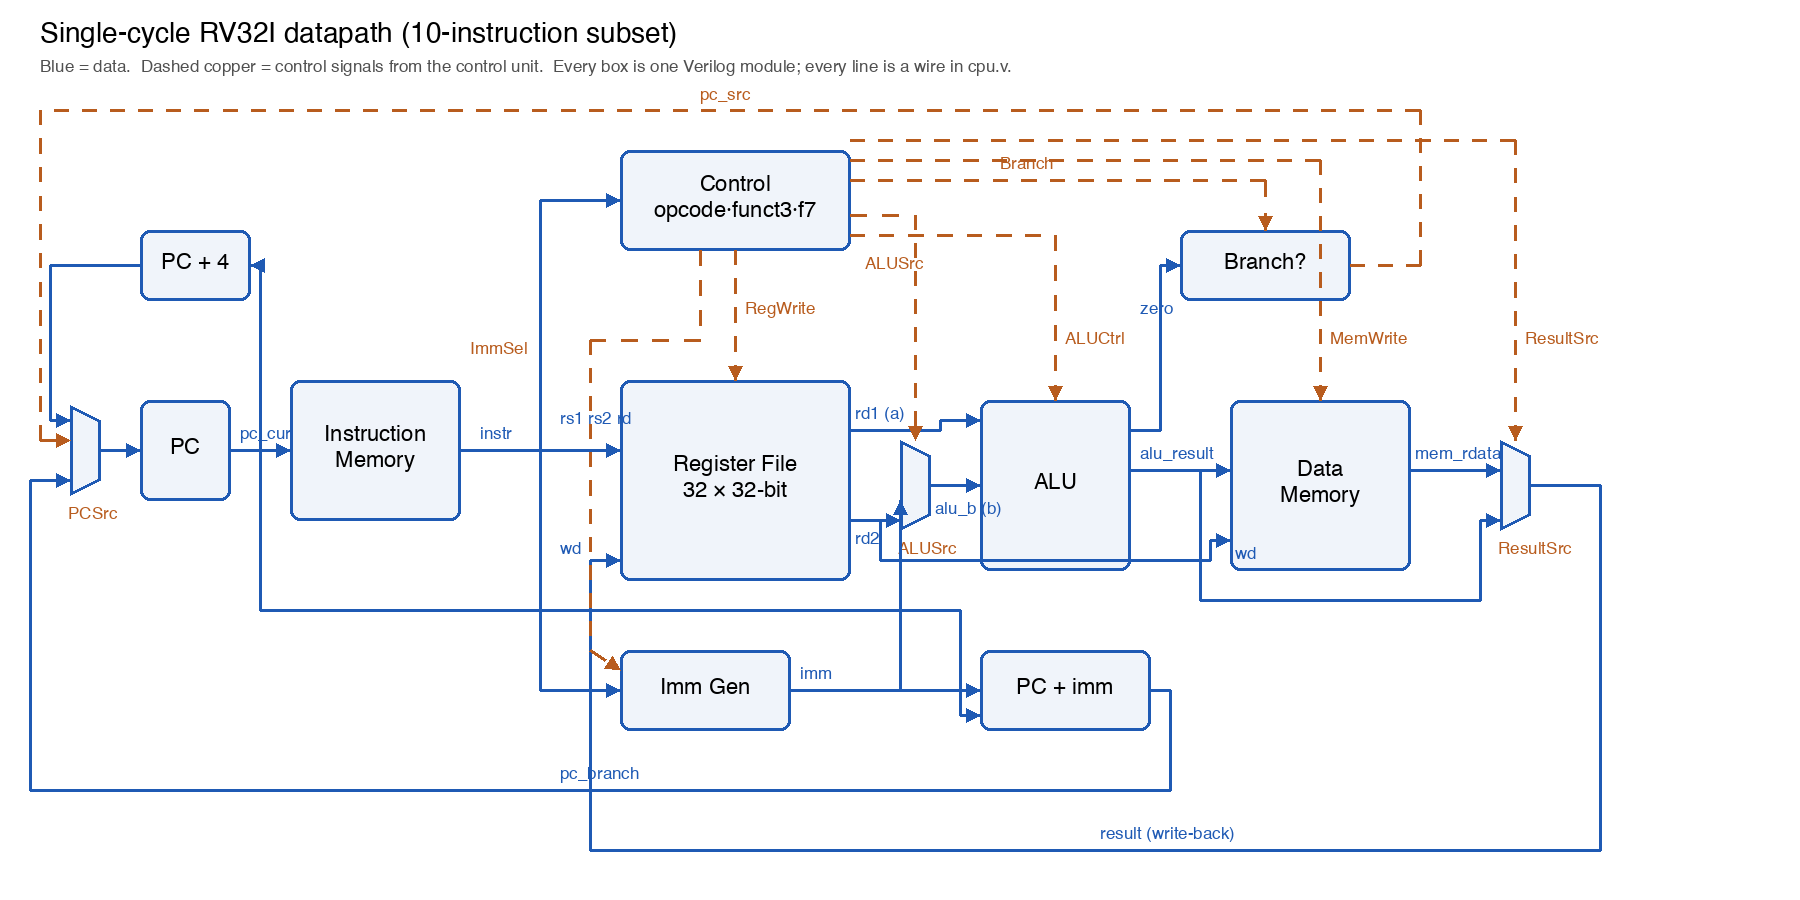
\includegraphics[width=\textwidth]{../docs/datapath.png}
\caption{Single-cycle RV32I datapath for the ten-instruction subset. Each box
is one Verilog module in \texttt{rtl/}; each line is a wire in
\texttt{cpu.v}. Solid lines carry data, dashed lines carry control signals
from the control unit.}
\label{fig:datapath}
\end{figure*}

\subsection{Instruction Set}
Table~\ref{tab:isa} lists the ten instructions with the opcode, funct3 and
funct7 values that the control unit decodes, and Table~\ref{tab:formats} shows
how the 32 bits are laid out in each format~\cite{riscv_unpriv_2026}. The
register-register (R) instructions share opcode 0110011 and are told apart by
funct3 and by bit 30, the only funct7 bit that differs within this subset: it
is 1 for SUB and 0 otherwise. The immediate (I) format carries a 12-bit
constant in bits 31--20 and is used both by ADDI (opcode 0010011) and by LW
(opcode 0000011). The store (S) format needs rs1, rs2 and an immediate, so the
constant is split into bits 31--25 and 11--7 to keep the register fields in
their usual positions. The branch (B) format is an S-type whose immediate bits
are permuted so that it encodes a byte offset in multiples of two; the
immediate generator inserts the implicit trailing zero. In every format rs1 is
at bits 19--15, rs2 at 24--20 and rd at 11--7, which is why the register file
in Fig.~\ref{fig:datapath} connects to the instruction word without any
decoding.

\begin{table}[h]
\centering\scriptsize\setlength{\tabcolsep}{3pt}
\caption{Supported instructions and their encodings (from \texttt{rtl/control.v})}
\label{tab:isa}
\setlength{\tabcolsep}{2pt}\begin{tabular}{llllll}
\toprule
Instr & Type & opcode & funct3 & f7[5] & Operation \\
\midrule
ADD  & R & 0110011 & 000 & 0 & rd = rs1 + rs2 \\
SUB  & R & 0110011 & 000 & 1 & rd = rs1 $-$ rs2 \\
AND  & R & 0110011 & 111 & 0 & rd = rs1 \& rs2 \\
OR   & R & 0110011 & 110 & 0 & rd = rs1 $|$ rs2 \\
XOR  & R & 0110011 & 100 & 0 & rd = rs1 $\oplus$ rs2 \\
ADDI & I & 0010011 & 000 & -- & rd = rs1 + imm \\
LW   & I & 0000011 & 010 & -- & rd = Mem[rs1 + imm] \\
SW   & S & 0100011 & 010 & -- & Mem[rs1 + imm] = rs2 \\
BEQ  & B & 1100011 & 000 & -- & if rs1 = rs2: PC = PC + imm \\
BNE  & B & 1100011 & 001 & -- & if rs1 $\neq$ rs2: PC = PC + imm \\
\bottomrule
\end{tabular}
\end{table}

\begin{table}[h]
\centering\footnotesize\setlength{\tabcolsep}{3pt}
\caption{Instruction formats (bit positions)}
\label{tab:formats}
\begin{tabular}{lcccccc}
\toprule
Type & 31--25 & 24--20 & 19--15 & 14--12 & 11--7 & 6--0 \\
\midrule
R & funct7 & rs2 & rs1 & funct3 & rd & opcode \\
I & \multicolumn{2}{c}{imm[11:0]} & rs1 & funct3 & rd & opcode \\
S & imm[11:5] & rs2 & rs1 & funct3 & imm[4:0] & opcode \\
B & imm[12$|$10:5] & rs2 & rs1 & funct3 & imm[4:1$|$11] & opcode \\
\bottomrule
\end{tabular}
\end{table}

\subsection{Control Unit}
The control unit is purely combinational and is split into two decoders,
following~\cite{harris2021digital}. The main decoder (Table~\ref{tab:control})
looks only at the opcode. Every output is first assigned zero and the matching
case then overrides the signals it needs, so no output is ever left undefined
and no latch is inferred; an unknown opcode therefore writes nothing and does
not branch. The main decoder also produces a two-bit internal \texttt{alu\_op}.
The ALU decoder (Table~\ref{tab:aludec}) turns \texttt{alu\_op} into the
three-bit \texttt{alu\_ctrl} code shared with the ALU: addresses for LW and SW
always add, branches always subtract, and R-type instructions consult funct3
and bit 30 of the instruction. ADDI is given its own \texttt{alu\_op} value
(11) rather than sharing the R-type path. In an I-type instruction bit 30
belongs to the immediate, so a negative constant such as $-8$ would otherwise
be decoded as SUB. The testbench \texttt{tb\_control.v} checks all ten
instructions and seven edge cases, including ADDI, LW, SW and BNE with
negative immediates and an unsupported opcode, against
Tables~\ref{tab:control} and~\ref{tab:aludec}.

\begin{table}[h]
\centering\scriptsize\setlength{\tabcolsep}{3pt}
\caption{Main decoder truth table (from \texttt{rtl/control.v})}
\label{tab:control}
\setlength{\tabcolsep}{2pt}\begin{tabular}{lccccccc}
\toprule
Instr & RegW & ALUSrc & MemW & ResSrc & Br & ImmSel & ALUOp \\
\midrule
R-type  & 1 & 0 & 0 & 0 & 0 & 00 & 10 \\
ADDI    & 1 & 1 & 0 & 0 & 0 & 00 & 11 \\
LW      & 1 & 1 & 0 & 1 & 0 & 00 & 00 \\
SW      & 0 & 1 & 1 & 0 & 0 & 01 & 00 \\
BEQ/BNE & 0 & 0 & 0 & 0 & 1 & 10 & 01 \\
other   & 0 & 0 & 0 & 0 & 0 & 00 & 00 \\
\bottomrule
\end{tabular}
\end{table}

\begin{table}[h]
\centering\footnotesize\setlength{\tabcolsep}{3pt}
\caption{ALU decoder (from \texttt{rtl/control.v})}
\label{tab:aludec}
\begin{tabular}{llllll}
\toprule
ALUOp & funct3 & funct7[5] & alu\_ctrl & Operation & Used by \\
\midrule
00 & -- & -- & 000 & add & LW, SW \\
01 & -- & -- & 001 & sub & BEQ, BNE \\
11 & -- & -- & 000 & add & ADDI \\
10 & 000 & 0 & 000 & add & ADD \\
10 & 000 & 1 & 001 & sub & SUB \\
10 & 111 & -- & 010 & and & AND \\
10 & 110 & -- & 011 & or  & OR \\
10 & 100 & -- & 100 & xor & XOR \\
\bottomrule
\end{tabular}
\end{table}

The branch decision is made in \texttt{cpu.v}:
$\mathrm{PCSrc} = \mathrm{Branch} \wedge (\mathrm{funct3}[0] \;?\; \neg\mathrm{zero} : \mathrm{zero})$,
so BEQ branches when the ALU subtraction gives zero and BNE when it does not.

\subsection{Module Design}

\begin{table}[h]
\centering\footnotesize\setlength{\tabcolsep}{3pt}
\caption{Verilog modules}
\label{tab:modules}
\begin{tabular}{llll}
\toprule
Module & Owner & File & Type \\
\midrule
pc      & M1 & rtl/pc.v      & sequential \\
cpu     & M1 & rtl/cpu.v     & top level (wiring) \\
alu     & M2 & rtl/alu.v     & combinational \\
regfile & M3 & rtl/regfile.v & combinational read, clocked write \\
immgen  & M3 & rtl/immgen.v  & combinational \\
control & M4 & rtl/control.v & combinational \\
imem    & M5 & rtl/imem.v    & combinational (read-only) \\
dmem    & M5 & rtl/dmem.v    & combinational read, clocked write \\
\bottomrule
\end{tabular}
\end{table}

\noindent\textbf{Program Counter and Top Level (\texttt{pc.v}, \texttt{cpu.v}):}
The program counter is a 32-bit register that takes the value zero on the
clock edge when reset is asserted and \texttt{pc\_next} otherwise. The top
level instantiates the other seven modules by port name, declares every wire
in Fig.~\ref{fig:datapath}, and implements the next-PC logic:
\texttt{pc\_plus4} and \texttt{pc\_branch} come from two separate adders, and
\texttt{pc\_src} is asserted when \texttt{branch} is set and the ALU zero
flag matches the condition selected by funct3 bit 0.

\medskip
\noindent\textbf{ALU (\texttt{alu.v}):}
% Insert in Proposed Solution -> Module Design.
The ALU is a combinational module with two 32-bit operands and a 3-bit
operation selector supporting ADD, SUB, AND, OR, and XOR. Arithmetic
retains the low 32 bits; unused selector codes produce zero, and every
case assigns the result to avoid a latch. A zero output indicates a zero
result, allowing the top-level branch logic to test equality after SUB.


\medskip
\noindent\textbf{Register File and Immediate Generator (\texttt{regfile.v}, \texttt{immgen.v}):}
The register file holds 32 registers of 32 bits. Both read ports are
combinational, so the operands are available in the same cycle as the
instruction, while the single write port updates on the rising clock edge when
\texttt{we} is set. Register x0 is never written and both read ports return
zero when register 0 is selected, as the specification requires. The
immediate generator rebuilds the constant from the instruction word for the
I, S and B formats, placing the bits in their arithmetic order and filling the
upper bits with copies of bit 31 so that negative constants, such as the
$-8$ byte offset of the backward branch in Program B, remain negative in 32
bits.

\medskip
\noindent\textbf{Control Unit (\texttt{control.v}):}
Two combinational always blocks implement the main decoder and the ALU decoder
described above. The five opcodes are named with local parameters, every
output has a default of zero, and the decoder tables in
\texttt{docs/control\_table.md} and in the RTL are kept identical.

\medskip
% ==============================================================================
% Section: Proposed Solution -> Module Design (Memory Subsystem)
% Owner: Member 5 (Balanagu Srikar) - Memory & Verification
% ==============================================================================

\noindent\textbf{Memory Subsystem (\texttt{imem.v}, \texttt{dmem.v}):} 
The processor implements a modified Harvard memory architecture with isolated instruction and data address spaces, preventing structural memory hazards during single-cycle \texttt{LW} execution. 
Instruction memory (\texttt{imem}) is a 64-word (256-byte) read-only asynchronous array populated at simulation initialization via \texttt{\$readmemh}. Instructions are indexed by discarding the lower two byte-offset bits (\texttt{addr[7:2]}). 
Data memory (\texttt{dmem}) provides 64 words of read/write storage, featuring combinational asynchronous read access for single-cycle load writeback and synchronous clock-edge writing conditioned upon the write enable (\texttt{we}) signal.


% ==============================================================================
% Section: Proposed Solution -> Verification Plan
% Owner: Member 5 (Balanagu Srikar) - Memory & Verification
% ==============================================================================

\subsection{Verification Plan}
\label{sec:verification}

Processor verification employed a layered, self-checking simulation methodology executed in Icarus Verilog and visualized using GTKWave. Testing progressed from unit-level module validation to full-datapath architectural verification under realistic machine code execution.

\subsubsection{Hierarchical Test Strategy}
The verification flow comprises two primary phases:
\begin{enumerate}
    \item \textbf{Unit Testbenches:} Independent self-checking harnesses for isolated modules: the Arithmetic Logic Unit (\texttt{tb\_alu.v}), the 32-register file (\texttt{tb\_regfile.v}), and the dual-stage control unit (\texttt{tb\_control.v}). Each unit test bench systematically applied exhaustive or randomized vectors checking boundary values, such as zero-register protection in \texttt{regfile} and arithmetic flags in \texttt{alu}.
    \item \textbf{Integrated System Testbenches:} The top-level testbenches (\texttt{tb\_cpu.v} and \texttt{tb\_cpu\_loop.v}) instantiate the integrated processor datapath alongside instruction and data memory memories, verifying cycle-by-cycle signal propagation, control hazard resolution, and architectural register-memory consistency.
\end{enumerate}

\subsubsection{Program A: Complete ISA Coverage Benchmark}
To guarantee complete coverage of the 10 target instructions within the RV32I base integer specification, \textbf{Program A} executes each instruction format in an interdependent operational sequence:
\begin{itemize}
    \item \textbf{Initialization:} \texttt{ADDI} populates baseline operands ($x_1 = 5, x_2 = 3$).
    \item \textbf{R-Type Arithmetic and Logic:} \texttt{ADD}, \texttt{SUB}, \texttt{AND}, \texttt{OR}, and \texttt{XOR} execute in succession, writing results into destination registers $x_3$ through $x_7$.
    \item \textbf{Data Memory Load/Store Round-Trip:} \texttt{SW} persists the value of $x_3$ (8) to memory address $0\times00$; \texttt{LW} retrieves the stored word into $x_8$, verifying single-cycle read-after-write coherence between memory and register writeback.
    \item \textbf{Conditional Control Flow:} \texttt{BEQ} compares equal registers ($x_3 == x_8 == 8$), taking a $+8$-byte forward branch to bypass an invalidation instruction ($x_9 \leftarrow 1$). Subsequently, \texttt{BNE} evaluates unequal registers ($x_1 \neq x_2$), taking another $+8$-byte forward branch past $x_{10} \leftarrow 1$.
    \item \textbf{Terminal State:} Execution concludes at target register $x_{11} \leftarrow 42$ before entering an idle self-loop (\texttt{BEQ} $x_0, x_0, 0$).
\end{itemize}
The automated harness verifies all architectural registers and memory locations against golden reference values, guaranteeing zero false passes.

\subsubsection{Program B: Iterative Accumulation Benchmark}
\textbf{Program B} computes the sum of the series $\sum_{i=1}^{5} i = 15$ over 19 executed instructions. This test specifically exercises:
\begin{itemize}
    \item Backward branch execution using a negative two's-complement immediate offset ($-8$ bytes via \texttt{BNE}).
    \item Repeated synchronous register writeback and asynchronous dual-port reading across iterative loop states.
    \item Word-aligned data memory storage with non-zero offset addressing (\texttt{SW} $x_1, 4(x_0)$).
\end{itemize}

Waveform dumps in Value Change Dump (\texttt{.vcd}) format were analyzed to inspect control path timing, hazard-free multiplexer selection, and memory read/write synchronization.


\subsubsection{Verification Results}
Table~\ref{tab:results} lists the result of running every testbench in the
repository with Icarus Verilog. Table~\ref{tab:programs} gives the executed
instruction counts measured in simulation. Synthesis, maximum frequency and
timing are Phase II work and have not been measured.

\begin{table}[h]
\centering\footnotesize\setlength{\tabcolsep}{3pt}
\caption{Testbench results (Icarus Verilog)}
\label{tab:results}
\begin{tabular}{lL{4.2cm}l}
\toprule
Test & What it checks & Result \\
\midrule
tb\_alu     & 542 vectors: add, sub, and, or, xor, zero flag, unused codes & PASS \\
tb\_regfile & write/read x5, write to x0 ignored, two simultaneous reads, we=0 ignored, negative value & PASS \\
tb\_control & 10 instructions plus 7 edge cases, all 7 outputs against the truth table & PASS \\
tb\_cpu     & Program A: x1--x11 and data word 0 after execution & PASS \\
tb\_cpu\_loop & Program B: x1 = 15, x2 = 6, x3 = 6, data word 1 = 15 & PASS \\
\bottomrule
\end{tabular}
\end{table}

\begin{table}[h]
\centering\scriptsize\setlength{\tabcolsep}{3pt}
\caption{Program execution (measured in simulation)}
\label{tab:programs}
\begin{tabular}{lcccc}
\toprule
Program & Instructions & CPI & Cycles & Halt PC \\
\midrule
A (test\_all)  & 12 & 1 & 12 & 0x38 \\
B (sum\_loop)  & 19 & 1 & 19 & 0x1C \\
\bottomrule
\end{tabular}
\end{table}

% ---------------------------------------------------------------------------
\section{Individual Contributions}
Table~\ref{tab:contrib} is taken from the Git history: every listed file was
committed only by its owner.

\begin{table}[h]
\centering\footnotesize\setlength{\tabcolsep}{3pt}
\caption{Individual contributions (from \texttt{git log})}
\label{tab:contrib}
\begin{tabular}{L{1.9cm}L{4.1cm}L{2.2cm}}
\toprule
Member & Files committed & Report sections \\
\midrule
M1 Shaik Junaid & rtl/pc.v, rtl/cpu.v, README.md, .gitignore, docs/datapath.png & Abstract, Introduction, Architecture, report assembly \\
M2 Siraparapu Shiva Sankar Mani Kanta & rtl/alu.v, tb/tb\_alu.v, tb/run\_alu.sh, docs/waveforms/alu.png & Literature Review part 1, ALU design \\
M3 Nakkina Lakshmi Praneeth & rtl/regfile.v, rtl/immgen.v, tb/tb\_regfile.v, docs/waveforms/regfile.png & Literature Review part 2, regfile/immgen design \\
M4 Rishik Chowdary Karuturi & rtl/control.v, tb/tb\_control.v, tb/run\_control.sh, docs/control\_table.md, docs/waveforms/control.png & Instruction Set, Control Unit \\
M5 Balanagu Sesha Srikar & rtl/imem.v, rtl/dmem.v, programs/*, tb/tb\_cpu.v, tb/tb\_cpu\_loop.v, tb/run\_cpu.sh, docs/waveforms/cpu.png & Verification Plan, memory design, References \\
\bottomrule
\end{tabular}
\end{table}

% ---------------------------------------------------------------------------
\bibliographystyle{IEEEtran}
\bibliography{member2_references,member5_references}

\end{document}
